% $Id: template.tex 11 2007-04-03 22:25:53Z jpeltier $

\documentclass{vgtc}                          % final (conference style)
%\documentclass[review]{vgtc}                 % review
%\documentclass[widereview]{vgtc}             % wide-spaced review
%\documentclass[preprint]{vgtc}               % preprint
%\documentclass[electronic]{vgtc}             % electronic version

\let\ifpdf\relax

%% Uncomment one of the lines above depending on where your paper is
%% in the conference process. ``review'' and ``widereview'' are for review
%% submission, ``preprint'' is for pre-publication, and the final version
%% doesn't use a specific qualifier. Further, ``electronic'' includes
%% hyperreferences for more convenient online viewing.

%% Please use one of the ``review'' options in combination with the
%% assigned online id (see below) ONLY if your paper uses a double blind
%% review process. Some conferences, like IEEE Vis and InfoVis, have NOT
%% in the past.

%% Figures should be in CMYK or Grey scale format, otherwise, colour 
%% shifting may occur during the printing process.

%% These three lines bring in essential packages: ``mathptmx'' for Type 1 
%% typefaces, ``graphicx'' for inclusion of EPS figures. and ``times''
%% for proper handling of the times font family.

\usepackage{mathptmx}
\usepackage{graphicx}
\usepackage{times}
\usepackage{url}

%% We encourage the use of mathptmx for consistent usage of times font
%% throughout the proceedings. However, if you encounter conflicts
%% with other math-related packages, you may want to disable it.

%% If you are submitting a paper to a conference for review with a double
%% blind reviewing process, please replace the value ``0'' below with your
%% OnlineID. Otherwise, you may safely leave it at ``0''.
\onlineid{0}

%% declare the category of your paper, only shown in review mode
\vgtccategory{Research}

%% allow for this line if you want the electronic option to work properly
\vgtcinsertpkg

%% In preprint mode you may define your own headline.
%\preprinttext{To appear in an IEEE VGTC sponsored conference.}

\usepackage[export]{adjustbox}

\usepackage{enumitem}
\setlist{noitemsep} % or \setlist{noitemsep} to leave space around whole list

\usepackage{listings}
\usepackage{color}

\definecolor{dkgreen}{rgb}{0,0.6,0}
\definecolor{gray}{rgb}{0.5,0.5,0.5}
\definecolor{mauve}{rgb}{0.58,0,0.82}
\definecolor{gray}{rgb}{0.4,0.4,0.4}
\definecolor{darkblue}{rgb}{0.0,0.0,0.6}
\definecolor{cyan}{rgb}{0.0,0.6,0.6}

\lstdefinelanguage{XML}
{
  morestring=[b]",
  morestring=[s]{>}{<},
  morecomment=[s]{<?}{?>},
  stringstyle=\color{black},
  basicstyle=\small,
  showstringspaces=false,
  tabsize=4,
  identifierstyle=\color{darkblue},
  keywordstyle=\color{cyan},
  morekeywords={xmlns,version,rdf,rdfs,my,owl}
  columns=flexible,
  breaklines=true,
  breakatwhitespace=true% list your attributes here
}


%% Paper title.

\title{Interactive Visual Analytics of Molecular Data in Immersive Environments via a Semantic Definition of the Content and the Context}

%% This is how authors are specified in the conference style

%% Author and Affiliation (single author).
%%\author{Roy G. Biv\thanks{e-mail: roy.g.biv@aol.com}}
%%\affiliation{\scriptsize Allied Widgets Research}

%% Author and Affiliation (multiple authors with single affiliations).
%%\author{Roy G. Biv\thanks{e-mail: roy.g.biv@aol.com} %
%%\and Ed Grimley\thanks{e-mail:ed.grimley@aol.com} %
%%\and Martha Stewart\thanks{e-mail:martha.stewart@marthastewart.com}}
%%\affiliation{\scriptsize Martha Stewart Enterprises \\ Microsoft Research}

%% Author and Affiliation (multiple authors with multiple affiliations)
\author{Mikael Trellet\thanks{e-mail: trellet@limsi.fr}\\ %
      \parbox{1.4in}{\scriptsize \centering Venise group \\ LIMSI-CNRS }%
\and Nicolas Férey\thanks{e-mail: ferey@limsi.fr}\\ %
     \parbox{1.4in}{\scriptsize \centering Venise group \\ LIMSI-CNRS }%
\and Marc Baaden\thanks{e-mail: baaden@smplinux.de}\\ %
     \parbox{1.4in}{\scriptsize \centering LBT \\ IBPC-CNRS}
\and Patrick Bourdot\thanks{e-mail: bourdot@limsi.fr}\\ %
     \parbox{1.4in}{\scriptsize \centering Venise group \\ LIMSI-CNRS }}%

%% A teaser figure can be included as follows, but is not recommended since
%% the space is now taken up by a full width abstract.
%\teaser{
%  \includegraphics[width=1.5in]{sample.eps}
%  \caption{Lookit! Lookit!}
%}

%% Abstract section.
\abstract{
Bringing together, in a unique immersive environment, visualization and analysis of scientific and complex data requires a thorough approach in order to fulfill scientists specific expectations. This approach needs to consider both the highly heterogeneous nature of data, the dynamic interactions between experts and data, as well as the large amount of data involved in scientific studies.
Whereas small and static scientific datasets can be quickly deciphered thanks to standard immersive tools such as 3D visualization softwares, bigger and dynamic datasets overcome the analytical capacity of these tools and require an efficient platform to manipulate them. We raise, through the example of the structural biology field, the need for an approach based on a high-level definition of the content (scientific data) and the context (immersive environments and interfaces) in order to setup a platform able to present to the user a dynamic and intelligent representation of his data. This classification will also provide new ways to interact with the data via intelligent and direct links. This approach is based on the semantic definition of all the concepts manipulated in the environments, either abstract or concrete, which allows for an adaptive and interactive experience of both visualization and analysis.
} % end of abstract

%% ACM Computing Classification System (CCS). 
%% See <http://www.acm.org/class/1998/> for details.
%% The ``\CCScat'' command takes four arguments.

\CCScatlist{ 
  \CCScat{Computer Graphics}{I.3.7}{Three-Dimensional Graphics and Realism}{Virtual Reality}
}

%% Copyright space is enabled by default as required by guidelines.
%% It is disabled by the 'review' option or via the following command:
% \nocopyrightspace

%%%%%%%%%%%%%%%%%%%%%%%%%%%%%%%%%%%%%%%%%%%%%%%%%%%%%%%%%%%%%%%%
%%%%%%%%%%%%%%%%%%%%%% START OF THE PAPER %%%%%%%%%%%%%%%%%%%%%%
%%%%%%%%%%%%%%%%%%%%%%%%%%%%%%%%%%%%%%%%%%%%%%%%%%%%%%%%%%%%%%%%%

\begin{document}

%% The ``\maketitle'' command must be the first command after the
%% ``\begin{document}'' command. It prepares and prints the title block.

%% the only exception to this rule is the \firstsection command
\firstsection{Introduction}

\maketitle

%% \section{Introduction} 


With the increasing complexity of scientific data experts have to manipulate, the need for platforms able to handle the data flow complexity is strong. It is particularly true in the field of structural biology. One major step in this field, the numerical simulation process, can now deal with very large and heterogeneous molecular structures. These structures can be sometimes composed of several millions of particles and consist of many different types of molecules, including the simulated cell environment. This overall complexity brings the need to go beyond standard visualization solutions and to move towards integrated systems where visualization and analysis can be merged. 

These integrated systems must be able to deal with heterogeneous data and to render them for the expert in a condensed working environment.
Immersive environments can play an important role for these integrated systems, providing both a better comprehension of the 3D structure of molecules, and new interaction techniques shortening the manipulation of the data by the experts.

Some initiatives took advantage of recent development in Virtual Reality to enhance some structural biology tasks. Visualization is the first and most obvious task that had taken advantage of new adaptive stereoscopic screens and immersive environments to plunged the experts at the really center of their molecules~\cite{van2000immersive,stone_immersive_2010,odonoghue_visualization_2010,hirst2014molecular}. Manipulation of structures during specific experiments of docking has also been improved thanks to the use of haptic devices and audio feedbacks to drive a simulation~\cite{ferey_multisensory_2009}. Despite these studies, no specific development has been made to setup an immersive platform where the expert could manipulate data coming from different sources to accelerate and improve the development of new hypotheses.

Today, the main process followed by the experts in structural biology studies still compartmentalizes the visualization of data and their analysis into two different and independent frameworks based on different tools.
This splitting can be partly explained by the significant differences between the data handled by the 3D visualization softwares and the analytical tools.
On one side, 3D visualization solutions like PyMol~\cite{delano_pymol_2002}, VMD~\cite{humphrey_vmd:_1996} or UnityMol~\cite{lv2013game} explore and manipulate 3D structures coordinates composing the molecular complex that will be displayed. The scene seen by the user will be composed of 3D objects reporting the overall shape of a particular molecule and its environment at a particular state. This scene is static if we are interested in only one state of the molecule but it is often dynamic since we observe a whole simulated trajectory of a molecule undergoing some energetic constraints over time.

Analysis tools, on the other side, take into input raw numbers, on various format and from various sources depending on the pipeline in which they are used. Their outputs are graphical representation of trends or comparisons between parameters or properties in a way that experts can quickly understand and use these information to guide their new hypotheses.
During the process that tries to decipher a scientific mechanism, and as we highlighted previously, experts constantly move from visualization tools to analysis tools and vice versa, wasting a precious time along the way.

A major improvement of today available tools would bring into play a scenario where the 3D visualization of a molecular event would be coupled to a monitoring of the properties evolution, sub-elements distance variations and simulation parameters progression into a single working environment. The expert would be able to see any action performed in one space (either 3D visualization or analysis) with a coherent graphical impact on the second space to filter or highlight the parameter or sub-ensemble of objects targeted by the expert.

\begin{figure}[htb]
  \centering
  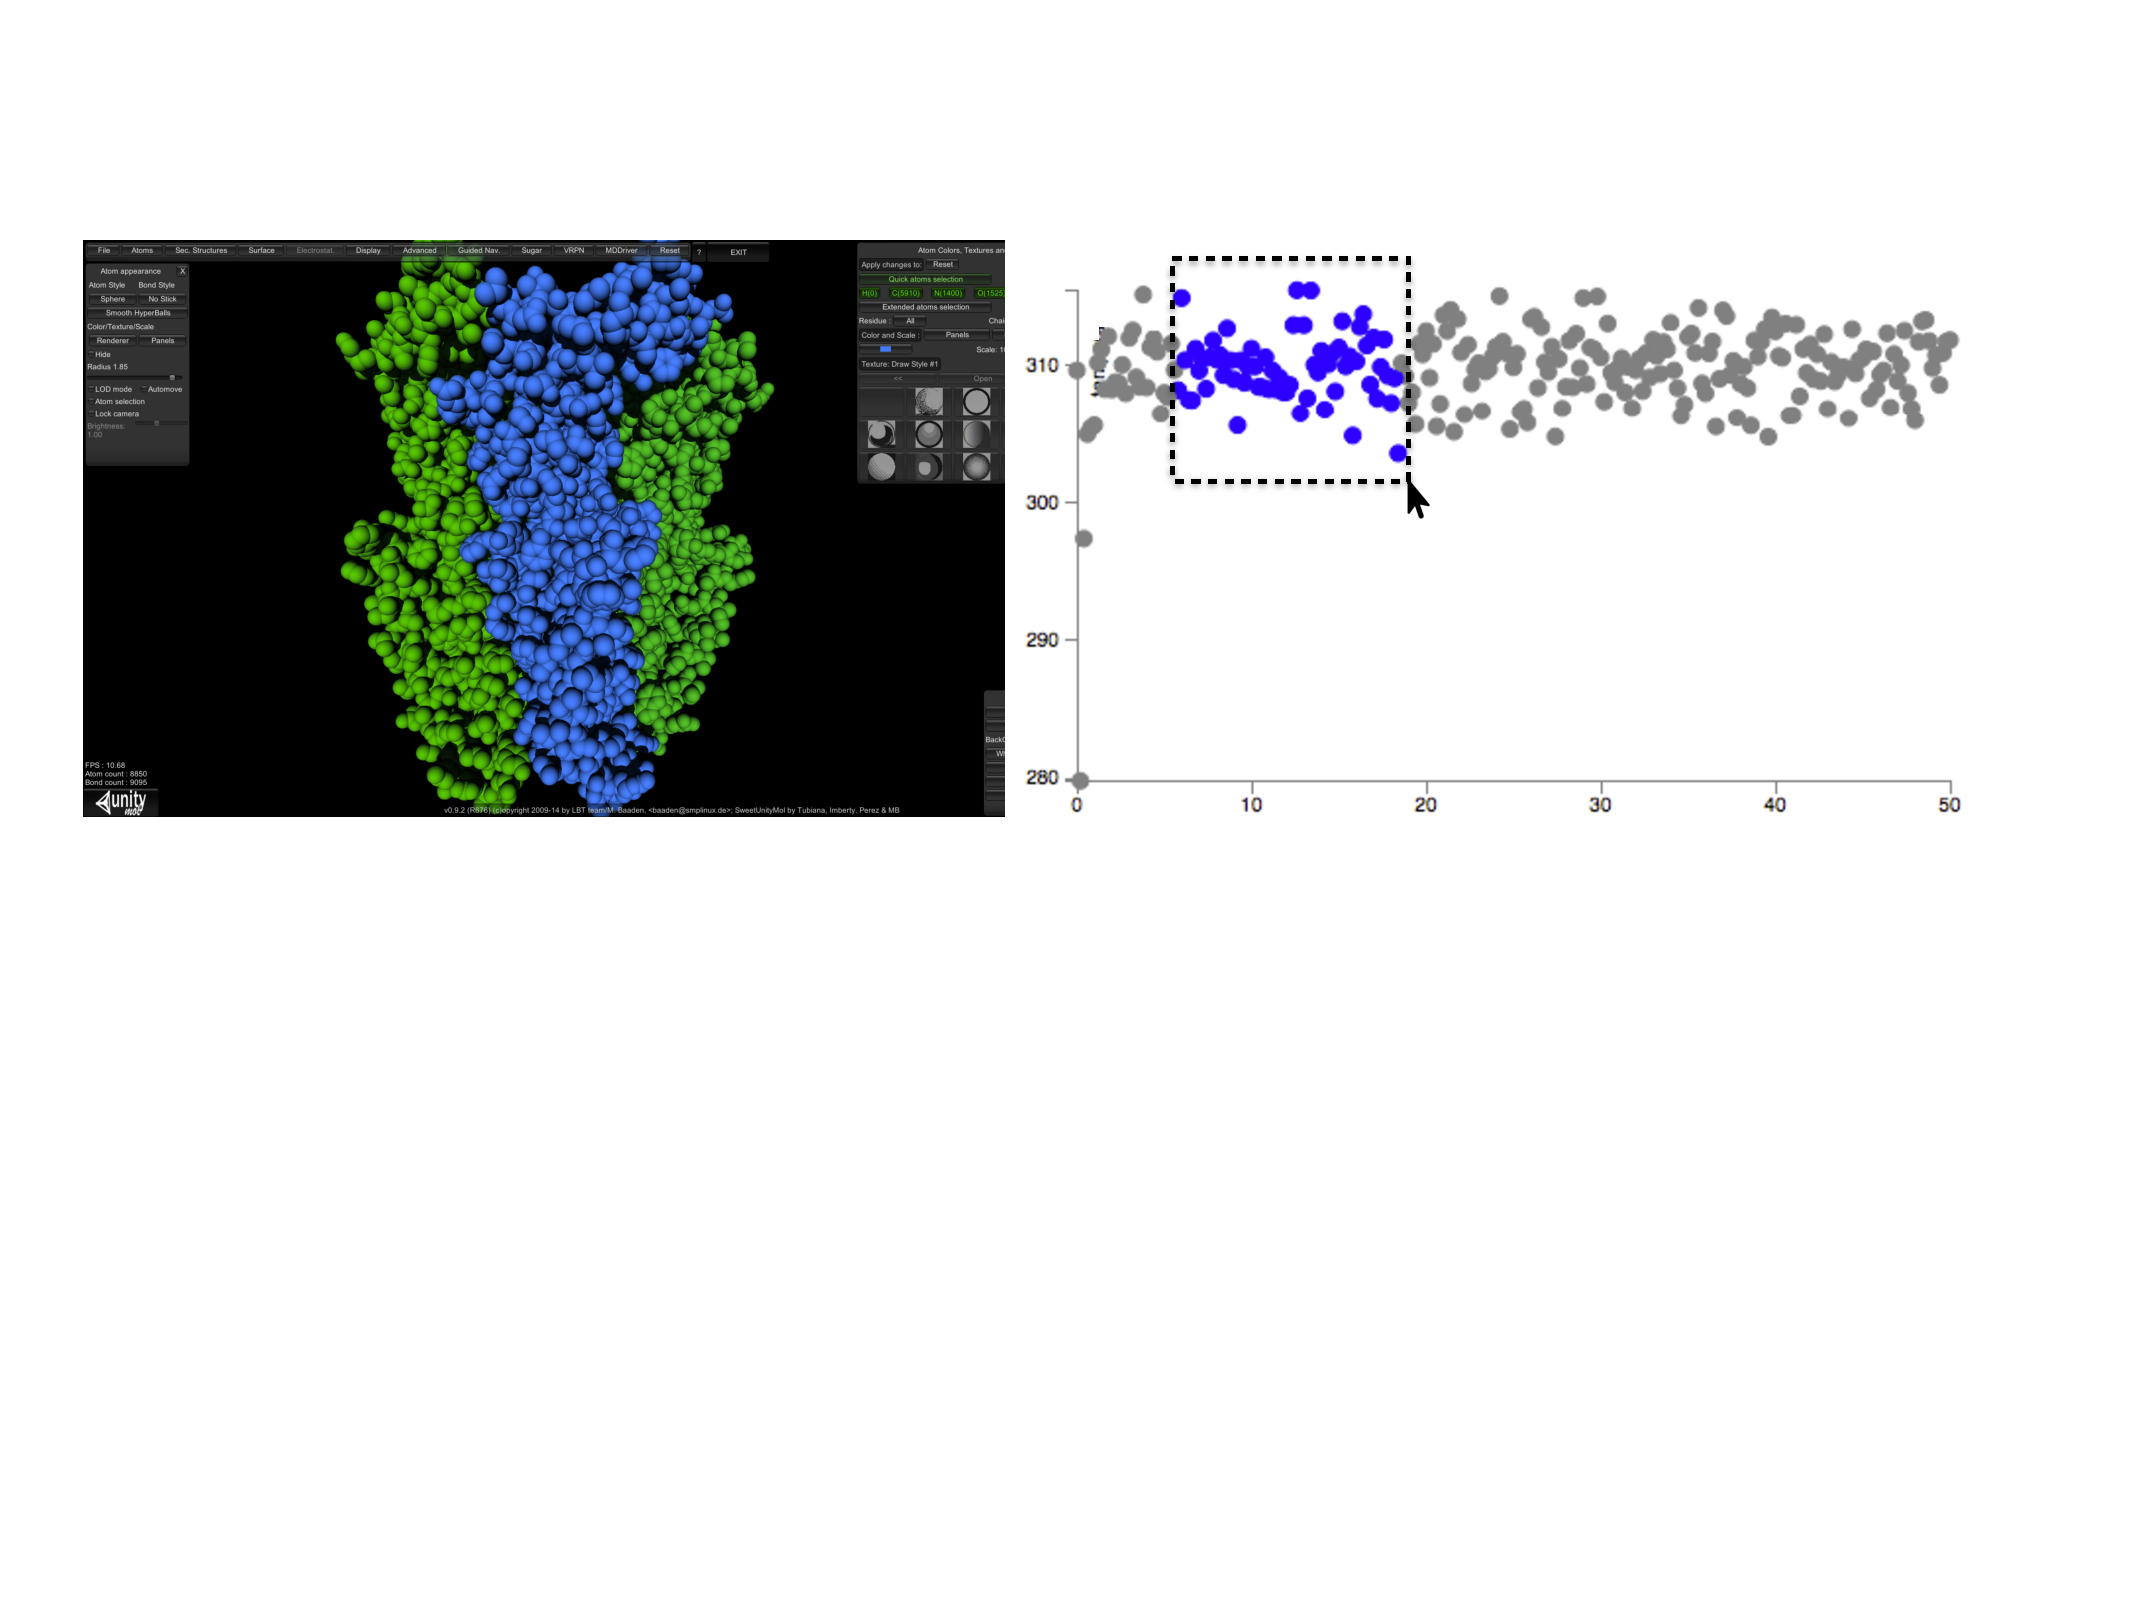
\includegraphics[width=\linewidth, frame]{figures/interactive_selection.pdf}
  \caption{3D visualization and analytical plot of a protein into two different spaces in the same environment. Any subset of points selected in the analytical space is instantaneously highlighted in the visualization space.}
  \label{interactive_selection}
\end{figure}

Immersive environments favor the combination of heterogeneous sources and provide several ways to merge data and processes for a particular task. But this combination of heterogeneous information brings a complexity not at the context level anymore but more at the content level. This complexity needs to be addressed in order to propose a fully-functional immersive environments where scientists will have the possibility to visualize, analyze and interact with their data.

There is a need to link heterogeneous data around an homogeneous framework where each object or group of objects can be related to the parameters or properties that define them. These links will first allow the access of an object by its parameters but, conversely, it will also allow the access of parameters by the object itself. And beyond the access, an interaction of the user with the graphical representation of either the object in the 3D visualization space, or the parameter in the analytical space, will have an impact in the reciprocal space as illustrated in the figure \ref{interactive_selection}.

A database defined by a high-level representation of all the data leads to an efficient way to mix visualization and analysis. By classifying knowledge, it is possible to create direct links between individuals and properties and then setup automatic retrievals of data each time an expert would need it.

The semantic definition of the application field can be enough to implement dynamic links between visual and analytical properties but do not allow for a specific way to interact with the data. As a result, we extended the definition of the structural biology content to the immersive context in which the platform will be used.
By doing so, we are able to combine information from both the expert knowledge and the user context in order to define intelligent interactions during the immersive working session.

% Bringing closer visualization and graphic analysis of scientific data while adding an interactive dimension is extensively studied in the field of Visual Analytics (VA). VA focuses on the graphical deciphering of complex data through interactive visual interfaces. This field stands on the border of several other fields such as the scientific visualization, the human-computer interaction and the perception with the aim to emphasize information that were previously hidden when using classic techniques from the cited fields in a partitioned way.

\section{Semantic definition of the platform}

In Computer Sciences, knowledge representation is often associated to the notion of ontology. An ontology is defined as a structured and hierarchical ensemble of concepts and relationships allowing to define a part or a whole field. An ontology must be comprehensible by both the computer systems and the humans. Indeed, an ontology often needs to be integrated into automatic processes and are setup by experts of a specific field, not always familiar with the computing side of the ontology.

Ontologies must allow the classification of any specific value or information into a pre-defined schema as instances of elements of this schema. It plays the role of a set of grammatical rules for a language made of data.
% For instance, a very simple ontology consisting of the two concepts "Atom" and "Charge" linked by a possessive relationship as illustrated in supplementary material.
% If any atom is added to a database defined by this ontology, an instance of the concept "Atom" will be created and a value of charge will be added to the property "Charge". The atom and the value will be linked and it will be possible to access them by searching either for the instance or for the property.

\subsection{State of the Art}

The semantic description of content through ontologies in immersive environments has been reported as a very efficient way to setup artificial intelligent systems ~\cite{Wiebusch:2015aa}, to design new VR applications~\cite{kleinermann2005designing} or to implement multimodal interactions~\cite{irawati2005semantic}. Although these developments allowed for a very interesting usage of semantic in immersive environments, they aim for a generic definition of either the content or the context and lack then either the expert field knowledge or the interactive possibilities, both required to setup intelligent interactions.

On the application side, the setup of ontologies in order to standardized knowledge in scientific fields has undergone an important and spontaneous growth at the end of the 90s~\cite{schulze-kremer_ontologies_2002}.

Bioinformatics, tightly anchored with structural biology, uses ontology for a long time. The most significant example is the genomic field where data flow quickly became unable to handle without a proper and standard organization of the data~\cite{schuurman_ontologies_2008}. \textit{Gene Ontology}~\cite{ashburner_gene_2000} was then created to regroup genomic data into a uniform format and databse and is now one of the most cited ontology. 
% Several biological databases or organizations like UniProtKB\footnote{\url{http://www.uniprot.org/uniprot/}} or the \textit{Open Biomedical Ontologies}~\cite{smith2007obo}, provide ways to access data or ontologies under RDF or OWL format to allow their use in expert tools or specific pipelines.

Only very few expert softwares in structural biology have based their development on the usage of ontologies. DIVE~\cite{rysavy_dive:_2014} and Avogadro~\cite{hanwell2012avogadro} appear both as exceptions, implementing, in different ways, a semantic description of the data they are manipulating. Avogadro is using the Chemical Markup Language (CML) to claim its semantic capability and add a description layer on top of the data the software is dealing with. However, no ontologies are setup and there is no use of the reasoning capabilities of this semantic description. 

DIVE offers the possibility to create on-the-fly ontologies and datasets based on the input data. This data representation allows a common data model that the software libraries will use. Then, creation of links between data values and concepts are possible and the different DIVE components (analyses, 3D visualization, etc.) are able to query them at any moment. Beyond value, links and relationships between the dataset elements can also be queried. DIVE implements then a powerful and generic ontology creator directly dependent on the type of data given as input. However, DIVE is limited to a quite simple reasoning on the ontology based on the multiple inheritance notion. It extends the basic oriented object philosophy found in JAVA, C\# or VB.NET for instance. Consequently, only some ontological relationships are available: \textit{is-a}, \textit{contains}, \textit{is-part-of} and \textit{bound-by}. There are no notion of cardinality or logical operators to define the concepts classes. Our needs are slightly more important and we identified several requirements that our approach should satisfy.


\subsection{Formalism choice}

The formalism of knowledge representation used in our approach must address these 3 rules to properly fit our platform needs:

\begin{enumerate}
  \item Hierarchical data representation via concepts and properties
  \item Reasoning possibility in order to extend the ontology or the dataset ruled by the ontology
  \item Efficient query time on the data to stay in interaction time
\end{enumerate}

Several formalisms exist to create ontologies and use them to define databases. A comparison of these formalism can be found in the table \ref{formalisms_comparison}.

\begin{table*}[t]
  % \centering
\begin{tabular}{l|*{5}{c|}}
Formalism          & Domain description & Reasoning on knowledge & Big data management & Efficient & Implementation flexibility \\
\hline
Conceptual Graphs  & X & X & - & X & -  \\
Semantic networks  & X & - & X & X & -  \\
Classical logics   & X & X & X & X & -  \\
Description logics & X & X & X & X & -  \\
\end{tabular}
\caption{Comparison of different knowledge representation formalisms with respect to key criteria.}
  \label{formalisms_comparison}
\end{table*}


We chose to use the Semantic Web approach in order to setup our own ontology. 
The Semantic Web has been created by the \textit{World Wide Web Consortium} under the lead of Tim Berners-Lee, with the aim to share semantic data on the web~\cite{berners2001semantic}. It is broadly used by the biggest web companies to uniformly store and share data. It belongs the family of the Description logics that uses the notions of \textit{concepts, roles} and \textit{individuals}. 
The \textit{concepts} are the sub-ensemble of elements in a specific universe, the \textit{roles} are the links between the elements and the \textit{individuals} are the elements of the universe~\cite{}. In our previous example, "Atom" and "Charge" would be \textit{concepts}, "has-a" a \textit{role} and the oxygen an \textit{individual}, as an instance of the \textit{concept} "Atom".
% Each layer of the Semantic Webs (ontology, experimental data, querying process, etc.) have been associated to a language or a format. The different layers and their associated formats are described in the figure~\ref{web_semantic_hierarchy}. 

\subsection{Semantic Webs layers}

The Resource Description Framework (RDF) is the basic model of Semantic Webs. It is a graph-based model aiming to describe in a formal way resources and their associated metadata. It is based on a knowledge representation from triples, a triple being the smallest knowledge division in RDF. Every data description is then an ensemble of triples including (\textit{subject}, \textit{predicate}, \textit{object})~\cite{godel1999bach}.

The \textit{subject} is the resource described, the \textit{predicate} represents a property attached to the resource and the \textit{object} may represent a resource or a data (being a value of the attached property). Any resource is identified by an URI (Uniform Resource Identifier) whereas a data is anonymous since it can be duplicated (numerical value, string, etc.). An example of a triple could be:
\\
(\textit{http://ontology.org/\#Pierre}, \textit{http://ontology.org/\#age}, \textit{xsd:int\^{}\^{}26})
\\
RDF has been quickly extended by a semantic layer in a model called RDF Schema (RDFS)~\cite{brickley2004rdf}. It defines classes, sub-classes, properties and sub-properties from which RDF resources will inherit. 

% \begin{figure}[htb]
%   \centering
%   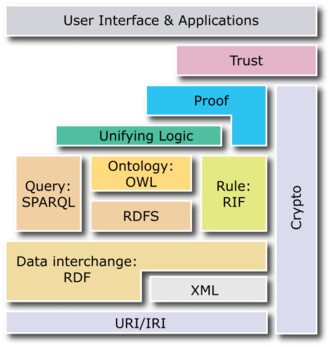
\includegraphics[width=.5\linewidth]{figures/web_semantic_hierarchy.png}
%   \caption{Hierarchical schema of the Semantic Webs multiple layer architecture}
%   \label{web_semantic_hierarchy}
% \end{figure}


% It permits the setup of relationships between high-level concepts and then extract relationships at the individual level. Included in the semantic layer, RDFS also provides the possibility to restrain the \textit{subjects} classes (\textit{rdfs:domain}) and \textit{objects} classes/datatypes (\textit{rdfs:range}) for a specific property used in RDF as a \textit{predicate}.
% For instance, the 2 following triples:
% \begin{lstlisting}[language=XML]
% <my:Protein>	<my:contains>	<my:Lysine>
% <my:contains>	<rdfs:range>	<my:Amino-acid>
% \end{lstlisting}
% \noindent
% will indirectly imply the following statement:
% \begin{lstlisting}[language=XML]
% <my:Lysine>	<my:is-a>	<my:Amino-acid>
% \end{lstlisting}
% \noindent

The semantic layer brought by RDFS can be complemented by another model named OWL. OWL is an computer standard, support of the Semantic Webs ontologies and grammatically defines RDF data to ensure their coherency and setup a semantic framework. It is complementary to the RDFS even if it goes further in terms of reasoning possibilities and resources description. More expressive than RDFS, OWL adds specific relationships based on logical links between properties or classes. It is then possible to add symmetrical, transitivity, similarity or cardinality information on top of concepts relationships.
Then, these triples:
\begin{lstlisting}[language=XML]
<my:is-composed-of>	<my:is-a>	<owl:TransitiveProperty>
<my:Protein>		<my:is-composed-of>	<my:Amino-acid>
<my:Amino-acid>		<my:is-composed-of>	<my:Atom>
\end{lstlisting}
will indirectly imply the following statement:
\begin{lstlisting}[language=XML]
<my:Protein>	<my:is-composed-of>	<my:Atom>
\end{lstlisting}

A crucial part of our immersive analytics platorm was to access the data defined by the ontology and stored as RDF triples. This access can be done efficiently via SPARQL, a query language and protocol used to access databases based on RDF triples. SPARQL allows not only to access data but also to edit, add or remove them. 
% The access is done thanks to a specific endpoint provided as an URL and accessible by most of software libraries handling RDF data. 
SPARQL is closely related to SQL in its functioning, implementing the SELECT, FROM, WHERE keywords for instance to build a query. 
% One of the difference with the SQL is the processing of queries. This is a 2-steps process where the first one is a research of matching patterns between the query and the database triples then a projection step where only the variables queries will be returned. 
Several operations are possible on the final results including SORT, JOIN, DISTINCT in order to filter or sort the results. Examples of SPARQL queries and results can be provided as supplementary material.

\section{Architecture}

The different layers introduced in the previous section needs to be setup in order to create a fully-integrated semantic layer around the immersive environment. Once this semantic definition is made, a core module will have the role to make the interface between the user actions, the data manipulated and the immersive environment.

\subsection{Ontology for the modeling of structural biology concepts}

Core of the platform, we implemented our ontology based on OWL and created a large description of concepts an expert would have to manipulate during visualization and analysis activities. We said previously that several bio-ontologies already existed. We extended one of them, a bio-ontology describing amino-acids and their biophysical and geometrical properties\footnote{\url{http://bioportal.bioontology.org/ontologies/AMINO-ACID}}.
Each component structuring molecular complexes and each associated property coming from various usual bio-informatics tools have been systematically defined in our ontology. However, since needs may vary, we designed this ontology to be easily updated and enriched with new concepts.
Our ontology has been designed around 5 categories, addressing 5 different parts of our platform:

\begin{itemize}
  \item \textbf{Biomolecular knowledge} - Gather field-related concepts and objects in structural biology 
  \item \textbf{3D representation} - Gather concepts related to the representation and visualization of 3D molecular complexes
  \item \textbf{2D representation} - Gather the concepts related to the representation of numerical analyses 
  \item \textbf{3D interactions} - Gather concepts related to the interactions in 3D environnements
  \item \textbf{2D interactions} - Gather concepts related to the interactions in 2D environnements
\end{itemize}

The separation of the categories does not induce that no relationship exist between two categories. For instance, "Atom" belongs to the \textbf{Biomolecular knowledge} category but is directly linked to the "Sphere" concept from \textbf{3D structure representation}. The whole network of connections will permit then to reason on the ontology in order to support the advanced interactivity level required in Visual Analytics.

Concepts and properties among the \textbf{3D representation} and \textbf{2D representation} categories gather the graphical elements that allow for the representation of \textbf{Biomolecular knowledge} category. Shape, colors but also graph types are notions defined in these two categories. 
% It is worth noting that analytical concepts are defined by graphical or abstract elements that play a role in the creation and visualization of an analytical result. However, we voluntarily chose to not define the different calculations and analyses of molecular simulation data because of their high complexity and their heterogeneous nature between the specialized tools. This does not mean that they will not be used among the platform, it is only not relevant to include them in the ontology.

In addition to the biomolecular concepts and representations previously cited, we also defined every concepts around the interaction between the user and the data he will directly or indirectly manipulate. These interactions include commands proposed by most of the visualization softwares and analysis tools.

\subsection{Molecular database}

Once we setup our ontology, it was possible to feed the database by adding biological information gathered by the expert. The new information will need to fit the vocabulary and classification defined by the rules present in the ontology in order to be adequately stored in the database.

The description of a molecular system goes through the analysis of any biological information that can be described by a character chain or a value and that correspond to a concept or property identified in the ontology. Each information will be exhaustively gathered in the RDF database as triples. Within the scope of our study, we focused on numerical molecular simulations. These simulations output at a regular time step a static snapshot of the molecular system. The energetic constraints of the simulation will make the system evolve towards specific states that experts try to decipher in order to understand some molecule mechanisms. The whole simulation creates then a trajectory where each state, at a precise time, is associated to a snapshot. A snapshot is defined in our ontology by the \textit{Model} concept. A \textit{Model} gathers all the atoms coordinates of the molecular system at a defined time step. In order to distinguish the different components of a system, these components are identified by \textit{Chain}, another concept of our ontology. Then, each \textit{Chain} in the system is composed of a sequence of \textit{Residues} (also known as \textit{Amino-acids} in proteins). The different inference rules present in the ontology allow us to not specify all the links between the different hierarchical component of a specific \textit{Model}. As a result, a \textit{Residue} that belongs to a specific \textit{Chain} will be automatically associated to the corresponding \textit{Model} where the \textit{Chain} appears.
Some triples of our database can be provided in supplementary material.

Every geometrical properties (position, angles, distance, etc.), physicochemical properties (solvant accessibility, partial charge, bonds, etc.) or analytical properties (energy, RMSD, temperature, etc.) are then integrated in the database and associated to individuals created from 3D structures (Model/Chain/Residue/Atom) for each step of the simulation. As a reminder, any individual are instance of concepts defined in the ontology. Individuals and their properties form then the population of the molecular database.

\subsection{Interrogation and queries for the direct interaction}

Once the data have been integrated in the RDF database, it is necessary to setup an interrogation system able to get back the data for their visualization and processing following interaction events in the working space. Our implementation of the query system mainly rests on the usage of SPARQL, as introduced before, and took several ways to address the different needs of our platform. SPARQL queries richness and flexibility allowed us to design an keyword to command interpretation engine that aim to transform a list of keywords into a comprehensive application command triggering an action in the working space.

One of the most adapted interactive technique in immersive environments is the vocal command. Based on a vocal recognition process, it consists of translating a sentence or a group of words said by the user into an application command. Vocal commands have the strong advantage to be associated with gestures to create multimodal commands.

Actions identified in our platform involve, for most of them, an action applied to a structural group designated by the expert. However, these structural groups can be characterized by: identifiers having a biological meaning (residues ids are, by convention, numbered from one extremity of the chain to the other), unique identifiers in the RDF database or via their properties.
The interpretation of commands vocalized by the expert with natural language and using a specific field-related vocabulary must go through a representation carrying the complexity of the knowledge and linking the objects targeted by the user to the virtual objects involved in the interaction.

To do so, we setup a process that will take as input a vocal command of the user and will translate it into an application command for the system. This can be summarized in 3 main parts:

\begin{enumerate}
  \item Recognition of keywords from a vocal command
  \item Keywords classification in a decomposed structure of command
  \item Creation of the final and operational command
\end{enumerate}

Our conceptualization effort and the use of the ontology mainly took place on the second part. Parts 1 and 3 are more implementation oriented and will not be deeply described.

\subsubsection{Keywords recognition}

The keywords recognition we are using is based on the keywords spotting capability of Sphinx~\footnote{\url{http://sourceforge.net/projects/cmusphinx/}}, a vocal recognition toolkit. Based on a dictionary created from the ontology list of concepts, it aims to detect any word said by the user that would match a word present in the dictionary.

\subsubsection{Keywords classification}

Each keyword recognized in the previous step is then assigned to a category. This classification is based on our ontology splitting which identifies 5 categories of word that can be found in a vocal command, semantically modeled:

\begin{itemize}
  \item \textbf{Action}
  \item \textbf{Component}
  \item \textbf{Identifier}
  \item \textbf{Property}
  \item \textbf{Representation}
\end{itemize}

This classification is done through successive SPARQL queries to the ontology. \textit{Action}, \textit{Component}, \textit{Property} and \textit{Representation} categories have their own concepts and can be identified by a unique word ("Hide", "Chain", "Charged", "Sphere", etc.). At the opposite, \textit{Identifier} category is linked to a concept instance from the \textit{Component} category. A biological identifier is very likely to be redundant because of the repetition of the molecular system at each time steps. The association between a component and an identifier in the keywords is then mandatory to detect any identifier and it is necessary that the component associated possesses the identifier in the database to validate the classification. 

SPARQL commands use the \textit{ASK} operator to define if a keyword belongs to a category or not. This operator takes one or several triples and return a boolean if the ensemble of triples is true or not with respect to the database. Some examples of queries can be found below:

\begin{lstlisting}[language=XML]
ASK {my:Hide rdfs:subClassOf my:Action}
ASK {my:Alanine rdfs:subClassOf my:Biological_component}
ASK {my:Cartoon rdfs:subClassOf my:Representation}
ASK {my:Aliphatic rdfs:subClassOf my:Property}
\end{lstlisting}

Reasoning and inference rules are automatically used in SPARQL queries and for instance, the following query:

\begin{lstlisting}[language=XML]
ASK {my:Alanine rdfs:subClassOf my:Biological_component}
\end{lstlisting}
\noindent
will output \textit{true} despite the absence of direct link between the two concepts (\textit{Alanine} and \textit{Biological\_component}) since \textit{AminoAcid}, \textit{Residue} and \textit{Molecule} are located between the two concepts (see Figure \ref{Fig:alanine_owl}).

\hspace{1cm}

\begin{figure}[!htb]
  \centering
  {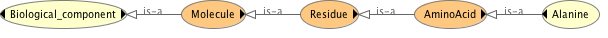
\includegraphics[width=\linewidth]{./figures/alanine_to_bio_component_owl}}
    \caption[Extract from OWL ontology for the \textit{Alanine} concept.]{\it Extract from our OWL ontology for the \textit{Alanine} concept.}
  \label{Fig:alanine_owl}
  % \hspace{0.3cm}
\end{figure}

Once each keyword is validated and associated to a category, e.g. identified as a concept of the database (or as an individual for identifiers) and eventually grouped with another keyword, it form a syntactic group. Each syntactic group carries an information which correspond to a specific part of the application command.

\subsubsection{From vocal command to application command}

In our platform, a vocal command is composed of syntactic groups succession linked between them to create an action query to the platform. It is possible to describe the type of command that we have defined in the following manner:

$$action\ [parameter]^+,\ (\ structural\_group\ [identifier]^+\ )^+$$

Syntactic groups between $[]$ are optional, at the opposite, others are mandatory. The $+$ indicates the possibility to have 0, 1 or several occurrences of the syntactic group. Finally, $()$ indicate a bloc of syntactic groups. This command architecture is present in our ontology under the form of pre-required concepts associated to the \textit{Action} concepts. For instance, the action concept \textit{Color} requires a property of \textit{Colors} type and a structural component to work with. These information are then stored in the ontology, making them automatically checkable by the engine to detect if all requirements are fulfilled for a specific action. This allows to have none or only slightly changes to bring to the engine when other actions are defined in the ontology. The checking process will stay the same as long as the action is well-defined in the ontology.

At the same level that an action, a structural group is always mandatory to trigger a command. The different ways to get a structural sub-ensemble are:

\begin{enumerate}
  \item Component only: Every individual that belongs to the concept will be taken into account
  \item Combination of a component and an ensemble of identifiers: 
  \item Property only: Every individual that possess the property will be taken into account
  \item Combination of a component and a property: Coherency checking between component and property
\end{enumerate}

The structural group always refers to a group of individuals in order to disambiguate the results between the commands. In return, the final command will be more complexed.
The hierarchical classification between structural components (Model/Chain/Residue/Atom) has a significant impact on a command effect. Indeed, the nature of structural components target by an action will be compared to the nature of the structural components currently studied. Depending whether the command individual will be of a higher or lower hierarchical order, the command might trigger an action on a subpart of the displayed scene (for lower classified individuals) or as a scene composition changer (for higher or equal classified individuals).
For instance, if only two models are studied when a vocal command is transmitted, putative amino-acids individual targeted by an action will be the ones that belong to the two displayed models. If the individuals target by the command action would have been models, different of the ones displayed, an update of the molecular complexes displayed would have occurred first.

Once the different checking for the command coherency and validity have been done, the command is sent to both spaces (visualization and analyses) in order to synchronize the visual results.

\section{Reasoning over semantic data - Scenario}

Our interpretation engine, able to translate a list of vocalized keywords into an application command is not the only possibility given by our semantic-based architecture. Any interaction of the user in either the visualization or analysis space with a structural group, a property or an analytic value is directly linked to an individual and its representations through the visualization or analytical filter. It is then possible to setup intelligent interactions in the immersive environment and synchronize any action of the expert between his two working spaces.

\subsection{Test case}

To illustrate the full-capacity of our platform, we chose a typical example of a molecular system study. This example setup a local visualization solution coupled to a distant web server where interactive graph can be created. Both spaces can be rendered in an immersive environment, either in the same screen space or split on one 3D screen for the visualization and a tablet for the web server. We assume, as it is the case in real studies, that the expert knows the molecular system and can interact vocally or by selecting elements in one of the space.

\begin{figure}[!htb]
  \centering
  {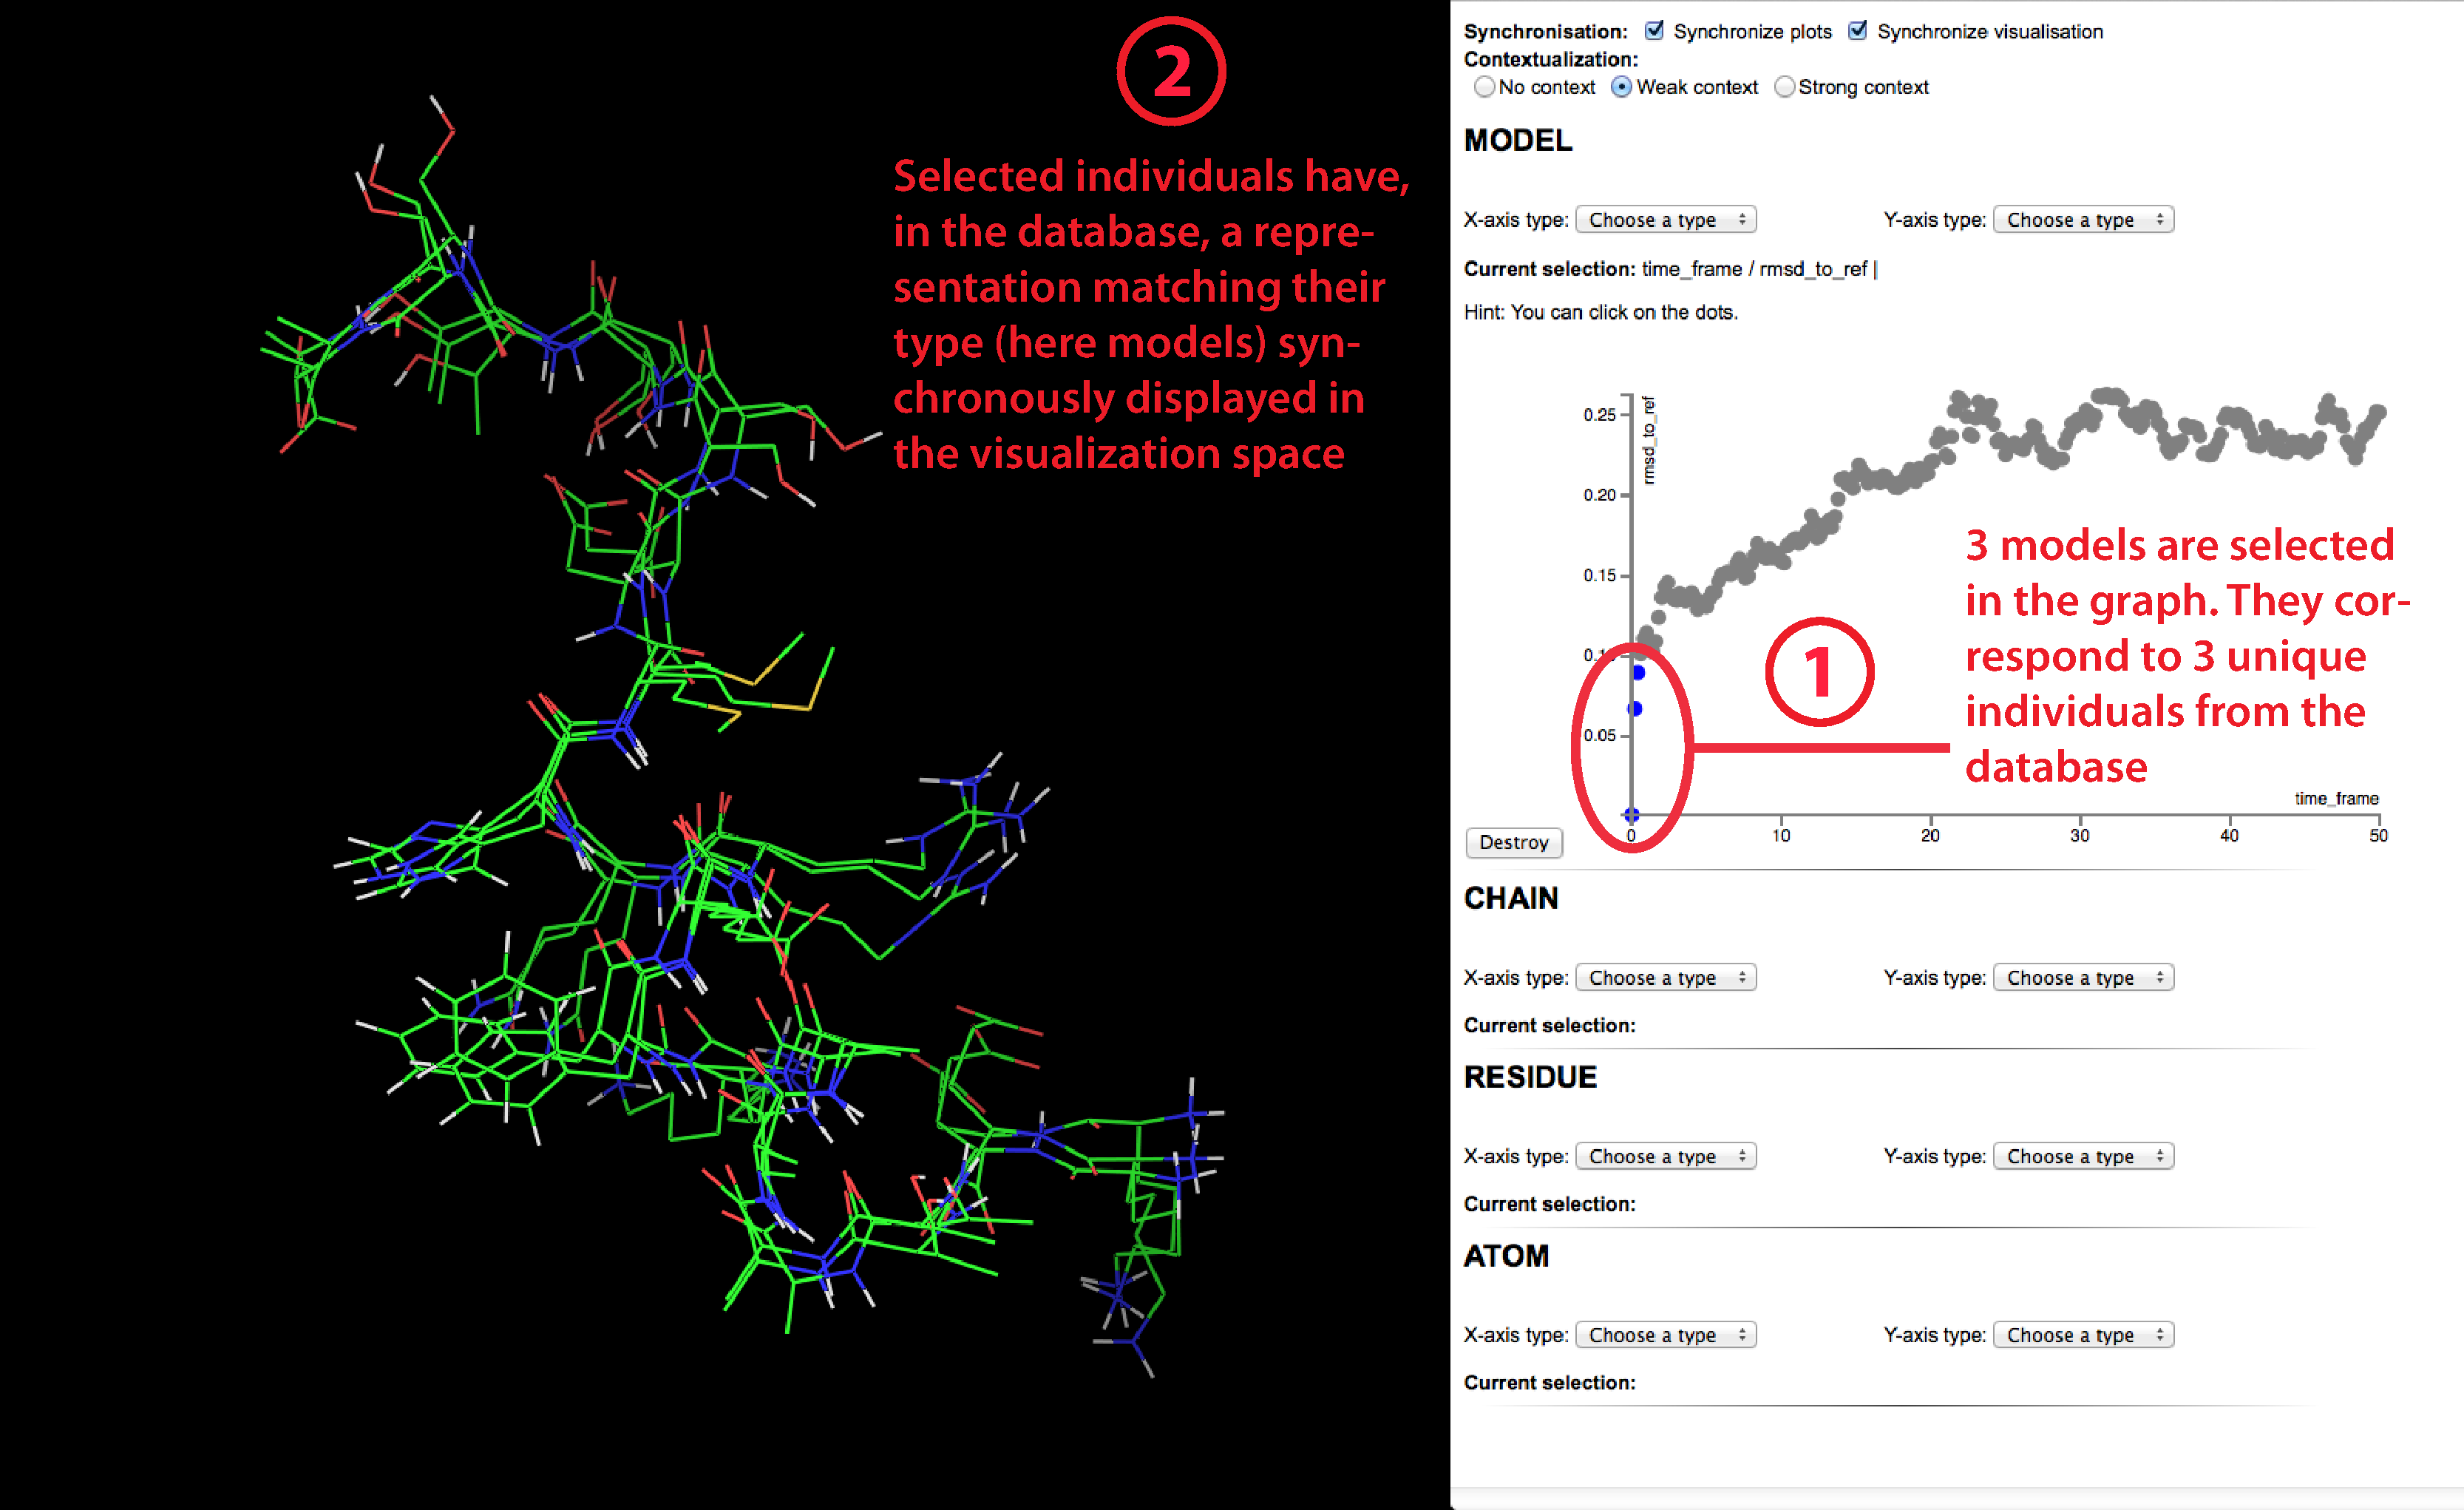
\includegraphics[width=\linewidth,frame]{./figures/scenario_step_1_cropped}}
    \caption[]{{\it On the right, selection of interesting models in the analytical space. The visualization state on the left is synchronized thanks to a SPARQL query in order to display the selected models.}}
  \label{Fig:1st_step}
  % \hspace{0.3cm}
\end{figure}

The first step of our scenario is a query triggered by the analytical space (web server) to get every numerical value that can be represented in a scatter plot. This will start the connection between the visualization space and the analytical space for the whole session. 
Once the values are gathered, the expert will choose which structural component hierarchy he is interested in and what combinations of properties he wants to plot. Several queries will get the property values and the web server graphs library, D3.js\footnote{\url{https://d3js.org/}}, will plot the values. We chose here to focus on the model level and display a criteria of distance between a reference model and all the models of the studied traject

The expert can select several models of importance, as shown in the first step of figure~\ref{Fig:1st_step}. The selection is synchronized over all the scatter plots previously created and will trigger a synchronous visualization of the individuals in the visual space (see second step of figure \ref{Fig:1st_step}).

Expert can then pass to the visualization space and select some elements of the displayed structures he would like to focus on. These sub-elements of the current models will be sent to the analytical space that will ask the expert for the properties to be plotted. Once the choice is made, the selection will be highlighted in the analytical space as shown in the figure \ref{Fig:2nd_step} for a selection of 3 residues.

The selection process can pass by a vocal command with our interpretation engine or by a manual selection. 
New graphs can be added on runtime at any moment and are synchronized with the current ones. However, it is important to note that a full synchronization between the visualization and analytical spaces requires the same hierarchy of structural elements selected in the spaces. If a new selection is done at a \textit{Model} level, any graphs of lower hierarchy will be reset with the new selected models and the visualization will be reset with the new models at the same time.

\begin{figure}[!htb]
  \centering
  {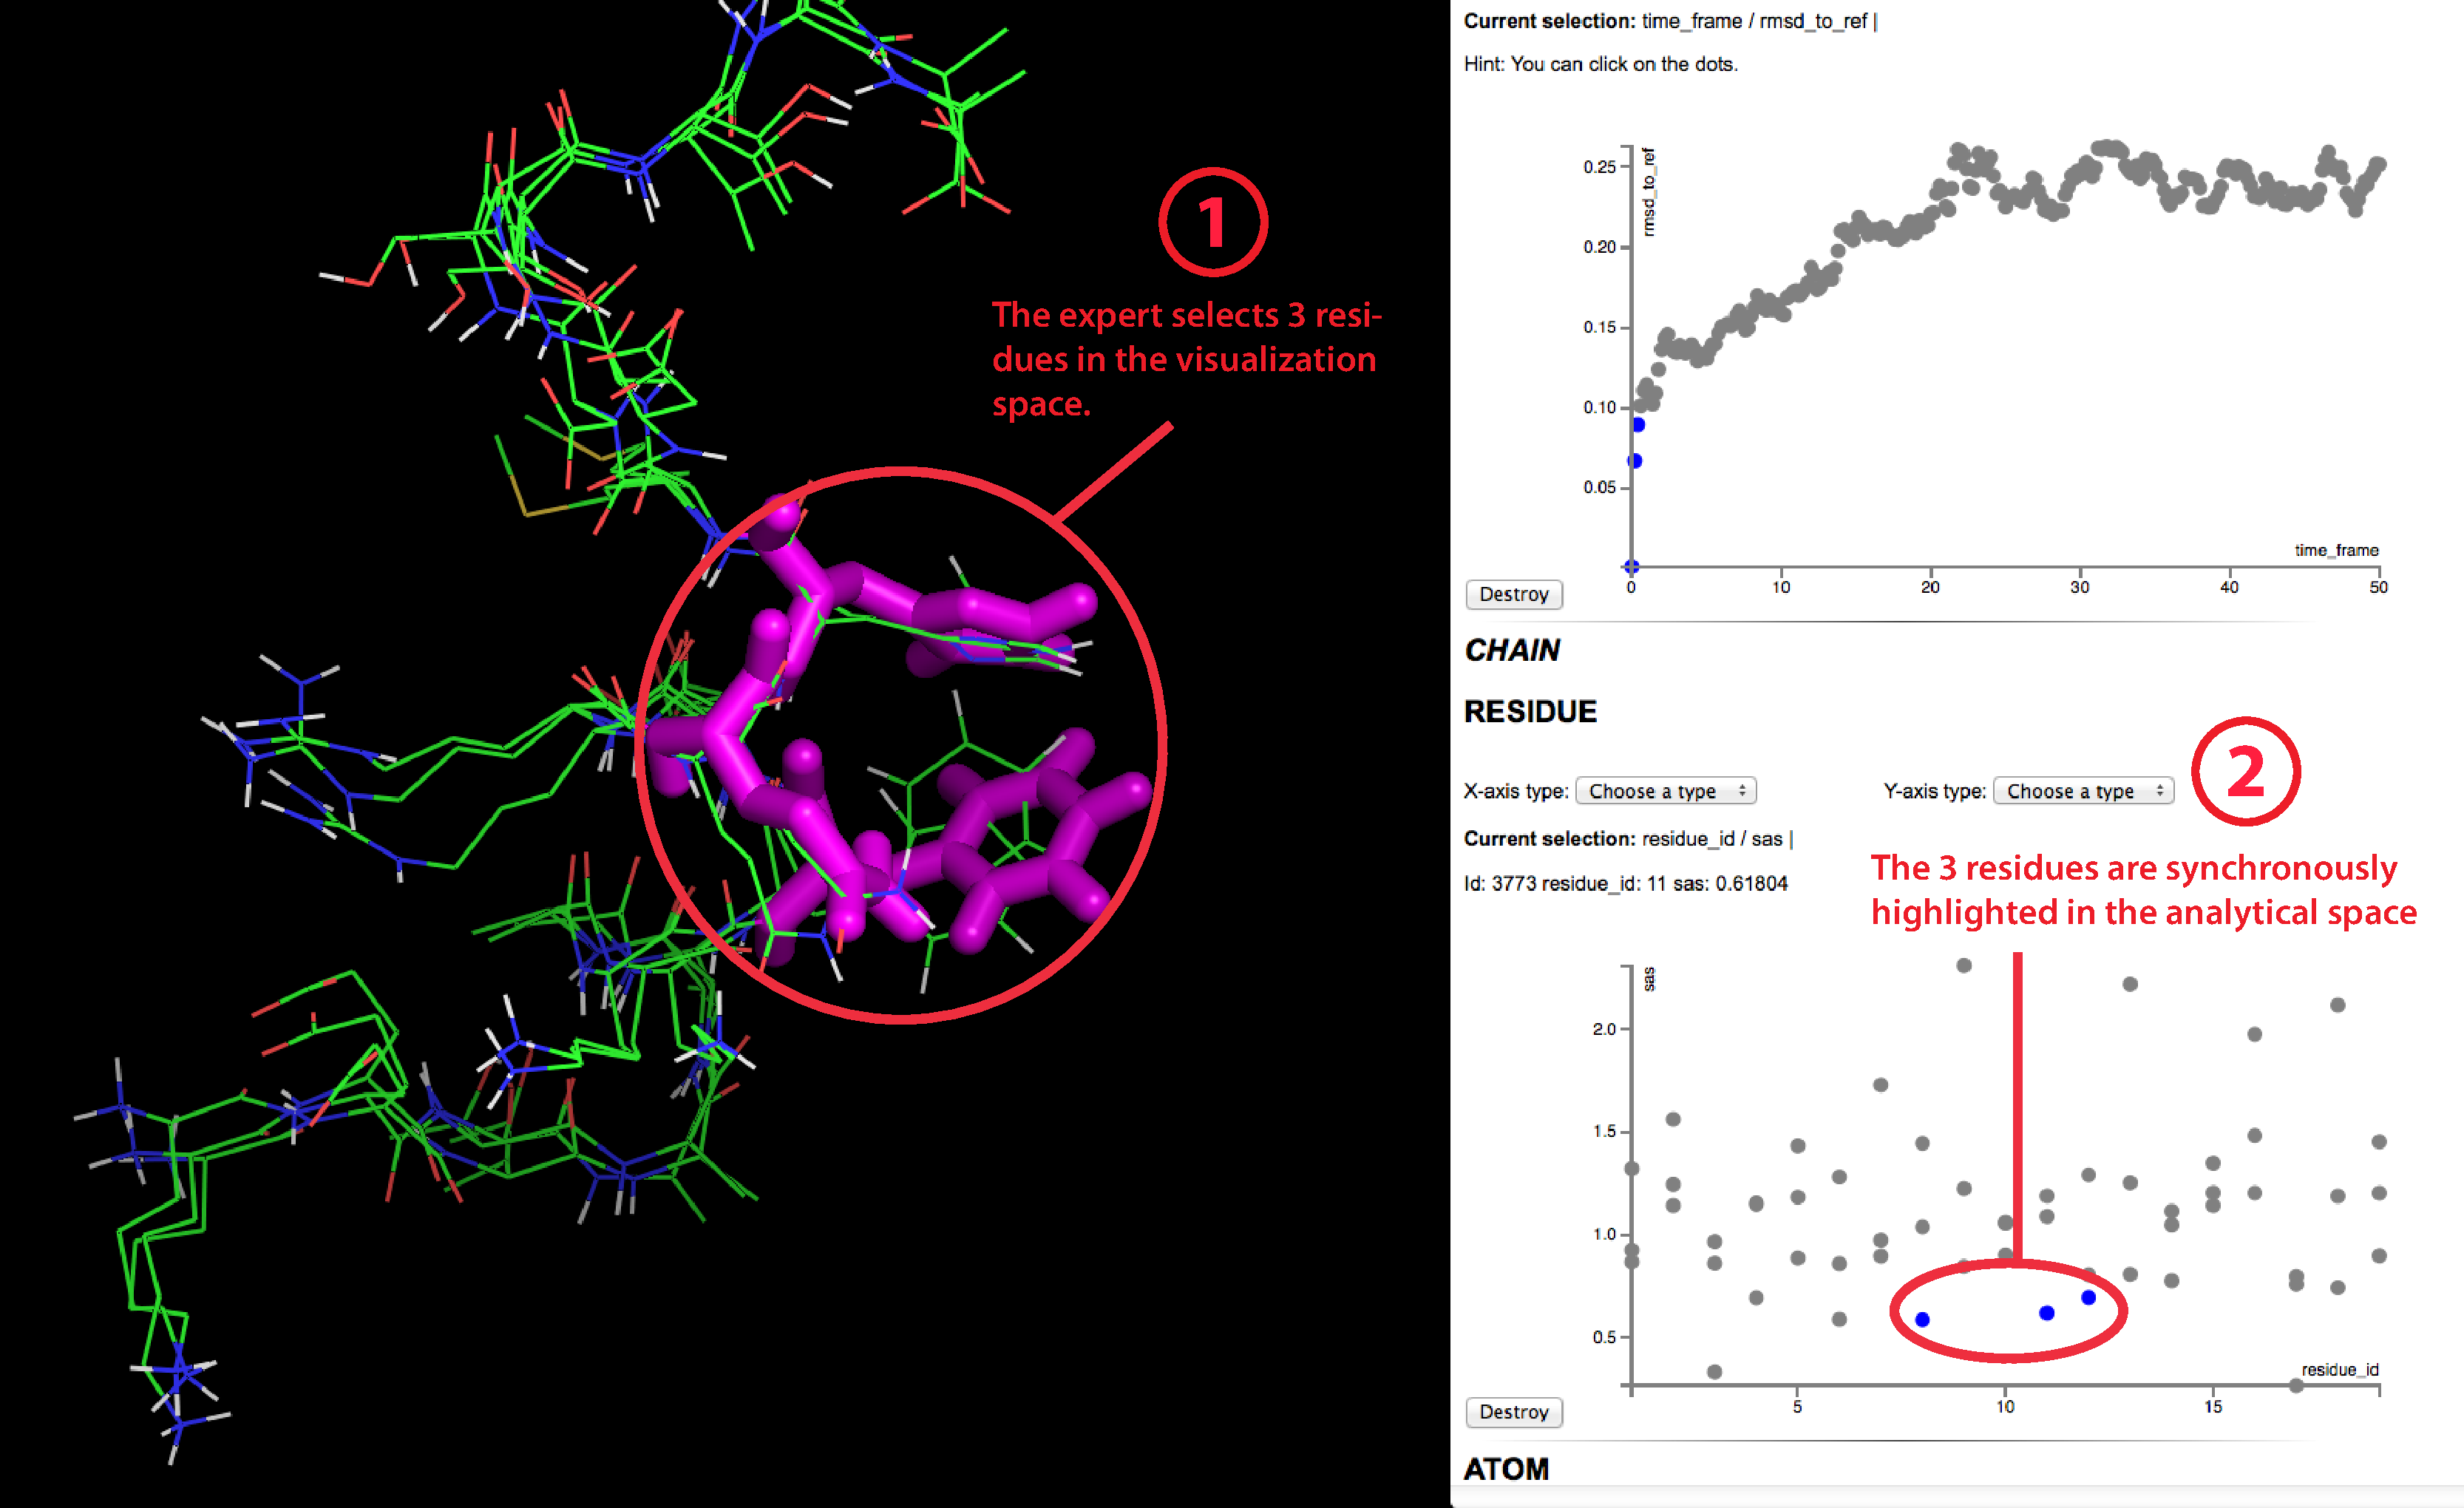
\includegraphics[width=\linewidth,frame]{./figures/scenario_step_2_cropped}}
    \caption[]{{\it On the left, selection of amino-acids of interest. The analytical space on the right is synchronized thanks to a SPARQL query and proposes adapted analyses to the expert.}}
  \label{Fig:2nd_step}
  % \hspace{0.3cm}
\end{figure}

\subsection{Evaluation}

The evaluation process started from the observation that the systematic evaluation of field-related tasks is rather complicated to setup because of: (1) usage and nature of the evaluated tools, in particular in molecular visualization, differ between experts. (2) implementation and adaptation of our developments over a representative sample of the tools is complex and very time-consuming. (3) Our approach is biased since based on the execution of expert tasks. (4) In order to apply standard statistic methods for evaluation, it is necessary to gather enough participants, the number of experts in our application field is rather limited.

We then propose an evaluation method more theoretical than empirical, the HTA method (for "Hierarchical Task Analysis")~\cite{annett2003hierarchical}. The HTA method consists in a division of a primary task into several sub-tasks. Each sub-task can be divided again until the sub-tasks reach a degree of precision sufficient to have their execution time evaluated accurately.

This method is particularly useful to compare similar tasks performed under different conditions. It allows to evaluate both the task methodology with respect to specific conditions and the performance of the conditions for a specific task. It requires only one expert to evaluate the different sub-tasks execution time.

\section{Conclusion}

We have setup a semantic layer over an immersive environment dedicated to the interactive visualization and analysis of molecular simulations data. This setup was done through the implementation of an ontology describing both structural biology and interaction concepts manipulated by the experts during a study process.

Our architecture, built around heterogeneous components, achieves to bring together visualization and analytical spaces thanks to a common ontology driven module that maintains a perfect synchronization between the different representations of the same elements in the two spaces.

The knowledge brought by the ontology can significantly improve the interactive capability of the platform by proposing to the user analyses adapted to the types of elements in his current focus. All along the study process, a set of specific analyses, non redundant with the ones already performed, can be interactively proposed to populate the database. A simple definition of analyses in the ontology, adding input and output types can decide if an analysis is pertinent or not for a precise selection and if the values are already present in the database.

The reasoning capability of the ontology allowed us to develop an efficient interpretation engine that can transform a vocal command made of keywords into an application command. This paves the way for a multimodal supervision tool that would use the high-level description of the manipulated elements, as well as the heterogeneous interaction natures, to fusion inputs and create intelligent and complex commands in line with the work of M.E. Latoschik~\cite{Wiebusch:2015aa} or~\cite{gutierrez2005semantics}.
The RDF/RDFS/OWL model coupled to the SPARQL language also allows to enunciate rules of inference, really important for the decision taking process in collaborative contexts. In these contexts, two users can trigger a multimodal command, in a conjoint way, that can be difficult to interpret without proper rules. An effort would have then to be made to integrate these rules in a future supervisor of the input modality, based on the semantic model, taken users as elements of modality in a multimodal interaction.

Our approach opens the way to a new generation of scientific applications. We illustrated our developments through the field of structural biology but it is worth to note that the generic nature of the Semantic Webs allows to extend our developments to most of scientific fields where a tight coupling between visualization and analyses is important. 


%% if specified like this the section will be ommitted in review mode
% \acknowledgements{
% The authors wish to thank A, B, C. This work was supported in part by
% a grant from XYZ.}

\bibliographystyle{abbrv}
%%use following if all content of bibtex file should be shown
%\nocite{*}
\bibliography{virtual_analytics}

% \section{Supplementary material}

% \subsection{SPARQL query example}

% \begin{lstlisting}[language=SPARQL]
% SELECT ?x ?id
% FROM <http://my_database.com> 
% WHERE {
%   ?y my:is-composed-of ?x .
%   ?y rdf:type my:Chain .
%   ?y my:chain_id "B" .
%   ?x my:res_id ?id
% }
% \end{lstlisting}
% \noindent

% \begin{center}
%  \begin{tabular}{|c | c|} 
%  \hline
%  ?x & ?id \\ [0.5ex] 
%  \hline
%  RES\_11 & 1 \\ 
%  RES\_12 & 2 \\
%  RES\_13 & 3 \\
%  RES\_14 & 4 \\
%  RES\_15 & 5 \\
%  \hline
% \end{tabular}
% \end{center}
% \noindent

% \subsection{Database triples}

% \begin{lstlisting}[language=XML]

% <owl:ObjectProperty rdf:about="&my;hasSize">
%     <rdf:type rdf:resource="&owl;FunctionalProperty"/>
%     <rdfs:domain rdf:resource="&my;AminoAcid"/>
%     <rdfs:range rdf:resource="&my;Size"/>
%     <rdfs:subPropertyOf rdf:resource="&my;has_property"/>
% </owl:ObjectProperty>

% <owl:DatatypeProperty rdf:about="&my;chain_id">
%     <rdfs:range rdf:resource="&xsd;int"/>
% </owl:DatatypeProperty>

% <rdf:Description rdf:about="my:ATOM_36795">
%   <my:atom_id rdf:datatype="#int">125</my:atom_id>
%   <my:time_frame rdf:datatype="#int">190</my:time_frame>
%   <rdf:type rdf:resource="my:Atom"/>
%   <my:pos_z rdf:datatype="#double">22.33</my:pos_z>
%   <my:atom_type>CB</my:atom_type>
%   <my:pos_x rdf:datatype="#double">21.86</my:pos_x>
%   <my:uniq_id rdf:datatype="#int">36795</my:uniq_id>
%   <my:pos_y rdf:datatype="#double">31.6</my:pos_y>
%   <my:belongs_to rdf:resource="my:RES_3622"/>
% </rdf:Description>

% \end{lstlisting}

\end{document}

